

\chapter{Experimental Apparatus}

This chapter describes the Large Hadron Collider (LHC) and the Compact Muon Solenoid (CMS) detector.


\section{The Large Hadron Collider}

Some of the parts of the Standard Model that we do not fully understand are the electroweak spontaneous symmetry breaking and the Higgs field.  As referred to in the previous sections, direct searches for the Higgs boson in the past have failed. The verification of the full Standard Model, including the discovery of the Higgs boson, is one of the main goals of physics.  Despite this being an important goal, the LHC has many other processes that it is sensitive to, including new physics. Figure~\ref{fig:lhcall} shows the predictions for some important Standard Model cross sections at  $p \bar p$ and  $pp$  colliders~\cite{Campbell:2006wx}. 

\begin{figure}[htb]                                                               
\begin{center}
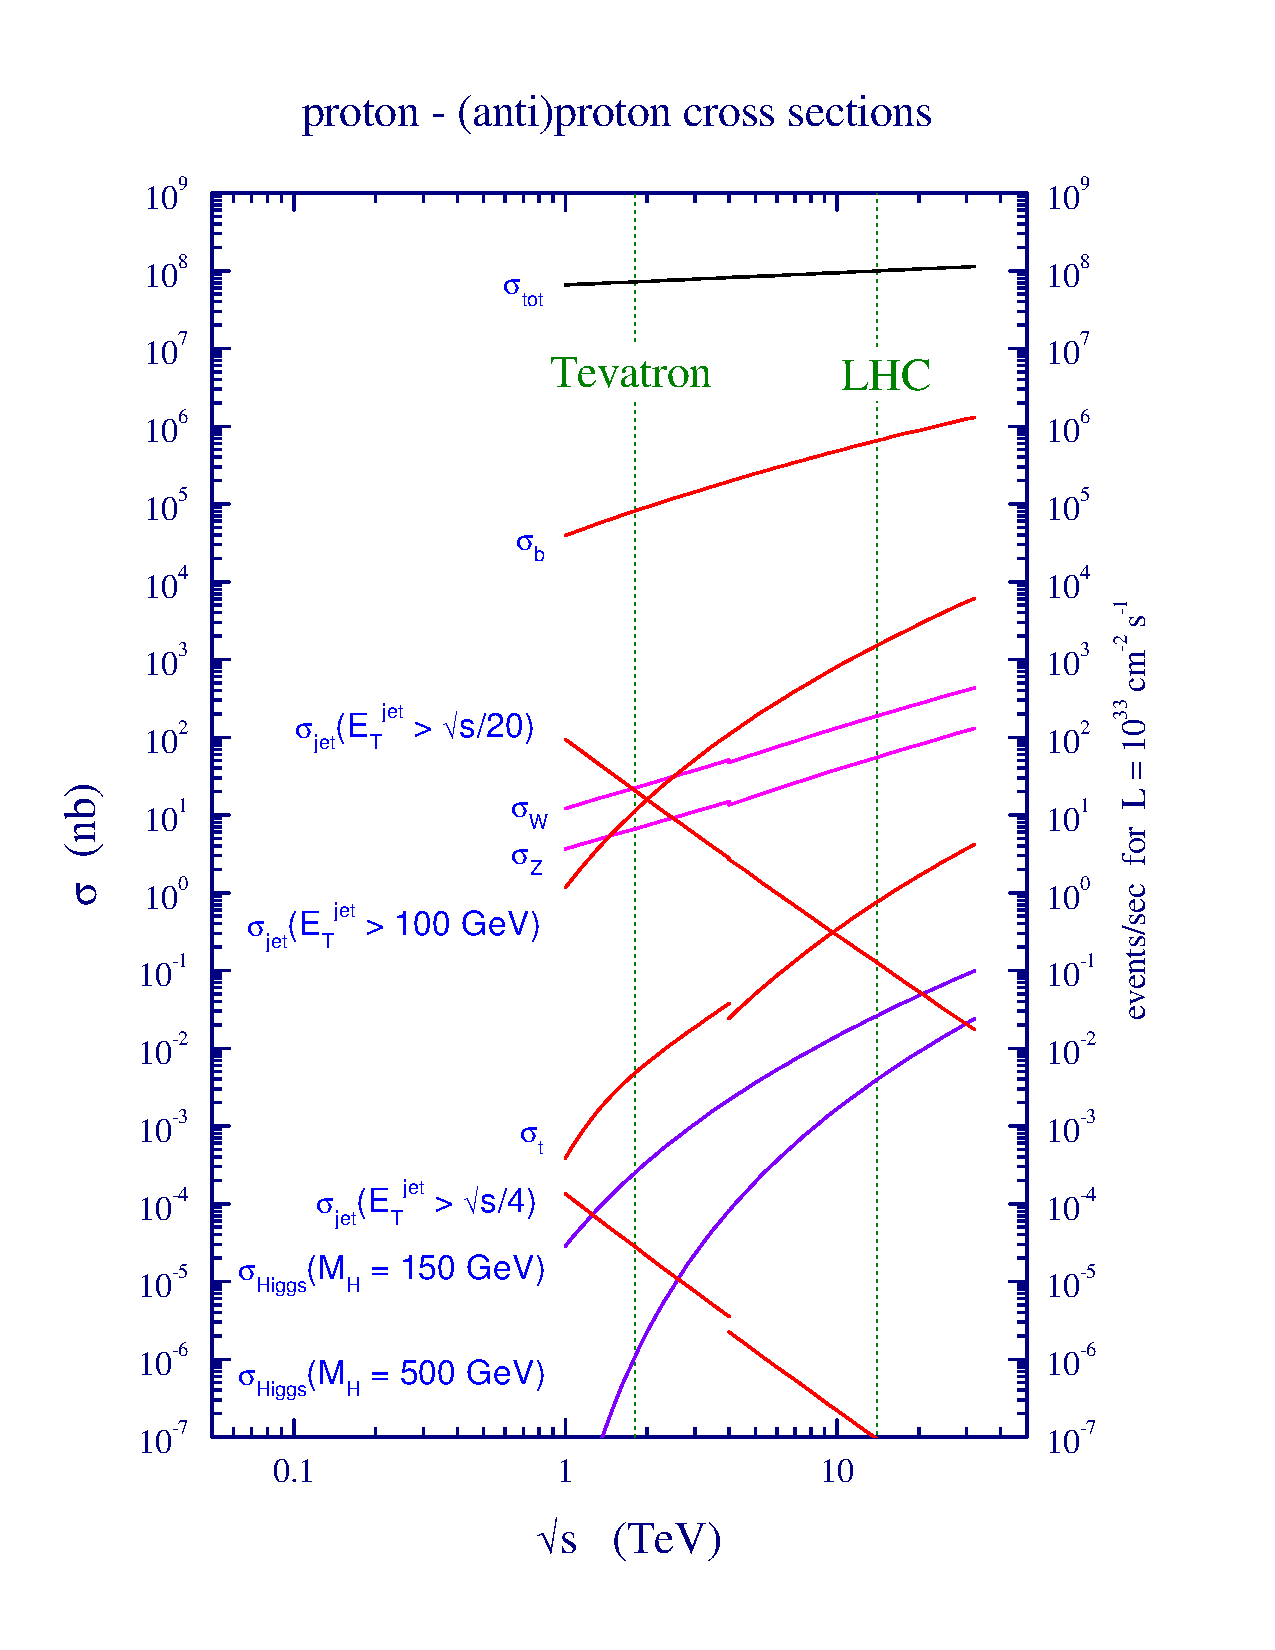
\includegraphics[width=0.99\textwidth]{Experiment/lhcolor.pdf}
\end{center}
\vspace*{-1cm}
\caption{Standard Model cross sections at the Tevatron
and LHC colliders.~\cite{Campbell:2006wx}}
\label{fig:lhcall}                    
\end{figure} 



The LHC accelerator is 26.7 km long and occupies the tunnel where the LEP collider was originally built.  This tunnel is located approximately 100 meters underground and spans the French and Swiss boarders near Geneva, Switzerland.  It is a proton-proton collider. The LHC is the world's largest and most powerful particle accelerator~\cite{LHCDesignReport}.

The LHC injection starts with a linear accelerator to bring protons to 50 MeV.  After the Proton Synchrotron (PS) accelerates them to 1.4 GeV, the Super Proton Synchrotron (SPS) then injects the protons into the LHC at an energy of 450 GeV.  To finish, the LHC increases the energy 0.5 MeV per cycle until they are at 4.0 TeV.  This can be seen schematically in Figure~\ref{fig:lhc_schematic}~\cite{CERN_complex}. The LHC can also accelerate lead ions.

\begin{figure}[htb]
\centering
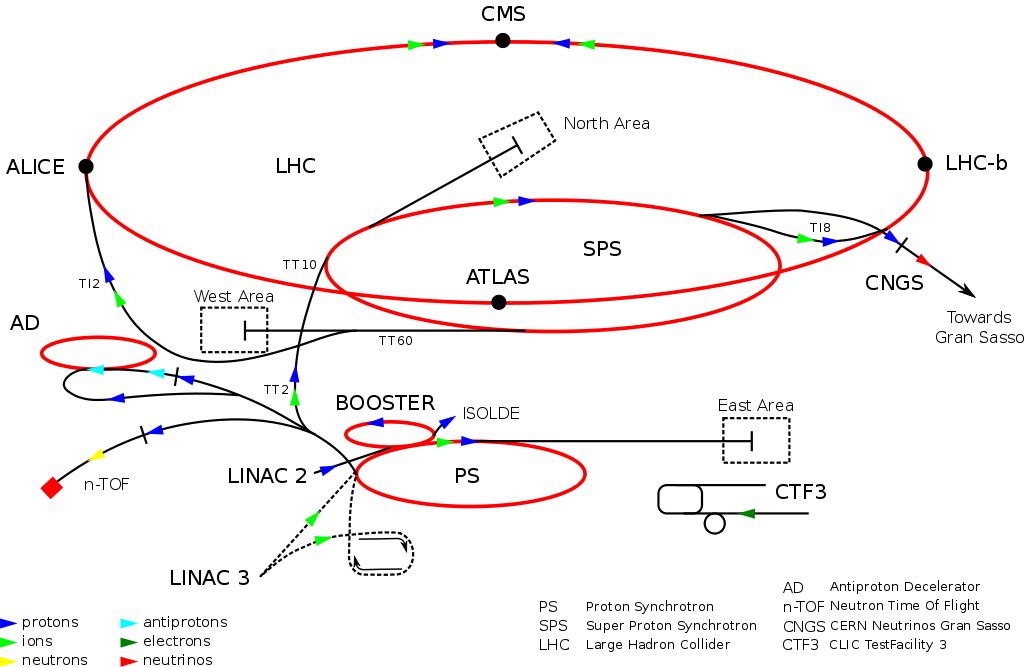
\includegraphics[width=0.99\textwidth]{Experiment/1024px-Cern-accelerator-complex.png}
\caption{Map of the CERN accelerator complex.\cite{CERN_complex}}
\label{fig:lhc_schematic}
\end{figure}

Because the protons being collided have the same electric charge, there are two vacuum chambers for acceleration with two different magnetic fields. There are 1,232 superconducting Niobium-Titanium magnets. Each one is 14.2 meters long and is cooled to 1.9 K with liquid Helium. The magnetic field produced is approximately 8.3 Tesla. These magnets are placed in 8 separate curved sections.

There are 4 interaction points in the LHC.  Two are high luminosity points at the general purpose experiments of A Toroidal LHC Apparatus (ATLAS) \cite{ATLASExperiment} and CMS. The other two are for the A Large Ion Collider Experiment (ALICE) \cite{ALICEExperiment}  and LHCb \cite{LHCbExperiment} experiments. These experiments can be seen in Figure~\ref{fig:lhc_experiments}.








\begin{figure}[htb]
\centering
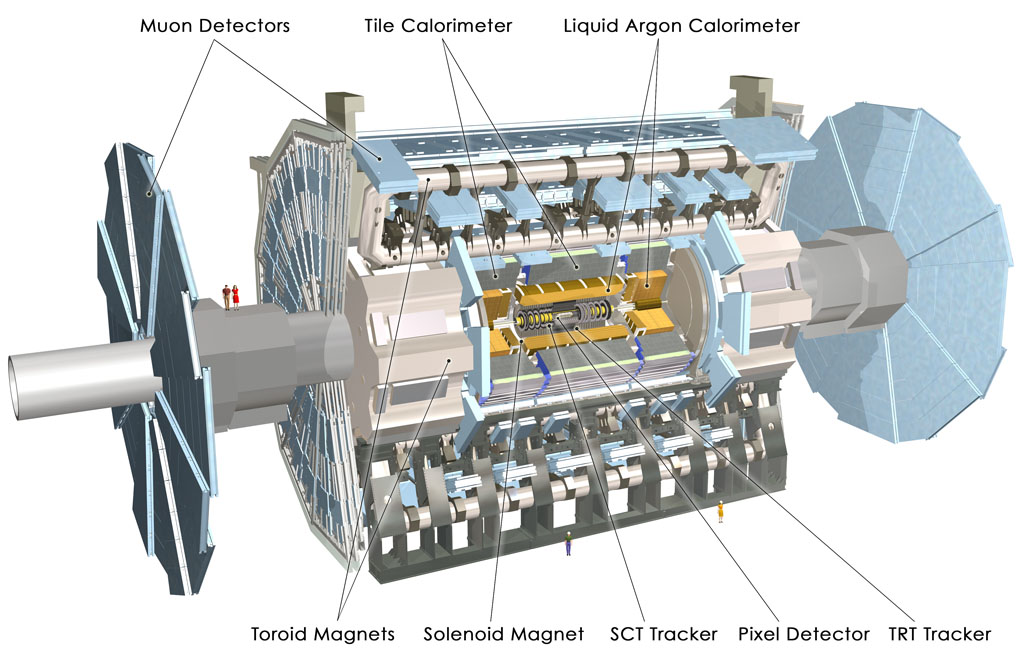
\includegraphics[width=0.49\textwidth]{Experiment/atlas.jpg}
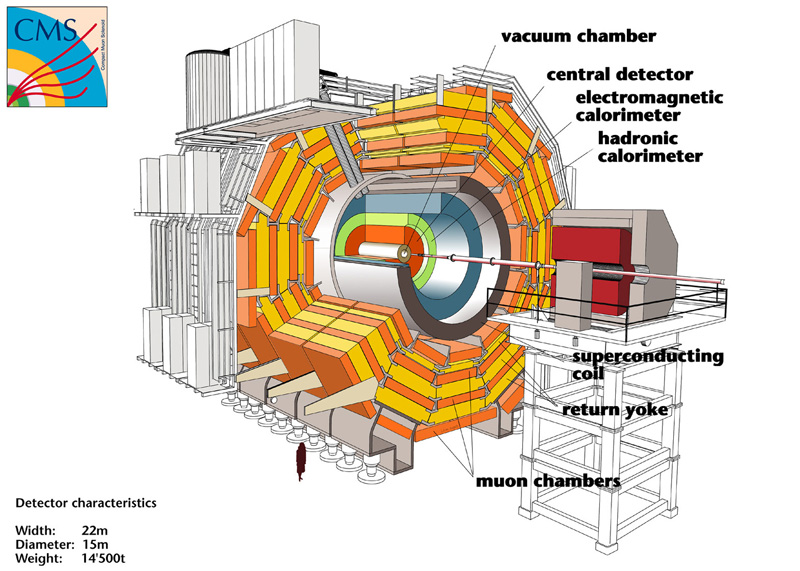
\includegraphics[width=0.49\textwidth]{Experiment/cms.jpg}
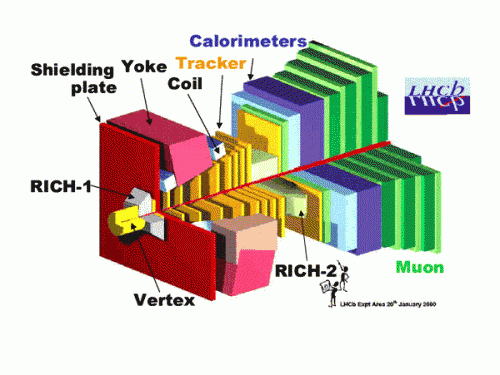
\includegraphics[width=0.49\textwidth]{Experiment/LHCb.png}
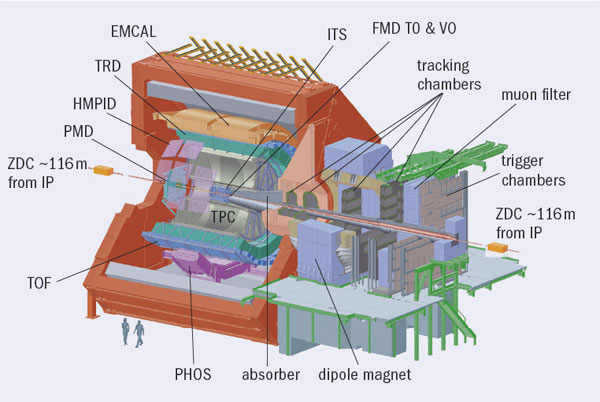
\includegraphics[width=0.49\textwidth]{Experiment/alice.jpg}
\caption{Top left: ATLAS experiment~\cite{ATLAS_image}. Top right:CMS experiments~\cite{CMS_image}. Bottom left: LHCb experiment~\cite{lhcb_image}. Bottom right: ALICE experiment~\cite{ALICE_image}.}
\label{fig:lhc_experiments}
\end{figure}




On November 23, 2009, the first proton-proton collisions were generated.  After a few runs at 450 GeV and 1.18 TeV beam energies, the first 7 TeV center-of-mass energies were achieved on March 30, 2010. This was the highest ever reached at a man-made particle collider.  At 7 TeV approximately 47 $pb^{-1}$ of integrated luminosity were delivered in 2010 (see Figure~\ref{fig:lhc_luminocity}). The maximum instantaneous luminosity was $2 \times 10^{32} cm^{-2}s^{-1}$.

During 2011 the machine was only off line for short amounts of time.  On October 26, 2011 the highest ever instantaneous luminosity was reached with a peak value of $3.5 \times 10^{33} cm^{-2} s^{-1}$.  This was 1,331 bunches per beam with collisions every 50 ns. The total integrated luminosity delivered was 5.73 $fb^{-1}$ (see Figure ~\ref{fig:lhc_luminocity}). In 2012 the beam energy was increased to 4 TeV and the LHC continued to perform amazingly, ultimately delivering over 23 $fb^{-1}$ (see Figure~\ref{fig:lhc_luminocity}).

In the coming years the LHC will continue to increase its energy and instantaneous luminosity.  Eventually it will reach larger energies around 13 TeV collisions and an instantaneous luminosity of $10^{34} cm^{-2}s^{-1}$.  This is seven times the energy of the highest Tevatron energy and two orders of magnitude more luminosity of any previous experiment.



\begin{figure}[htb]
\centering
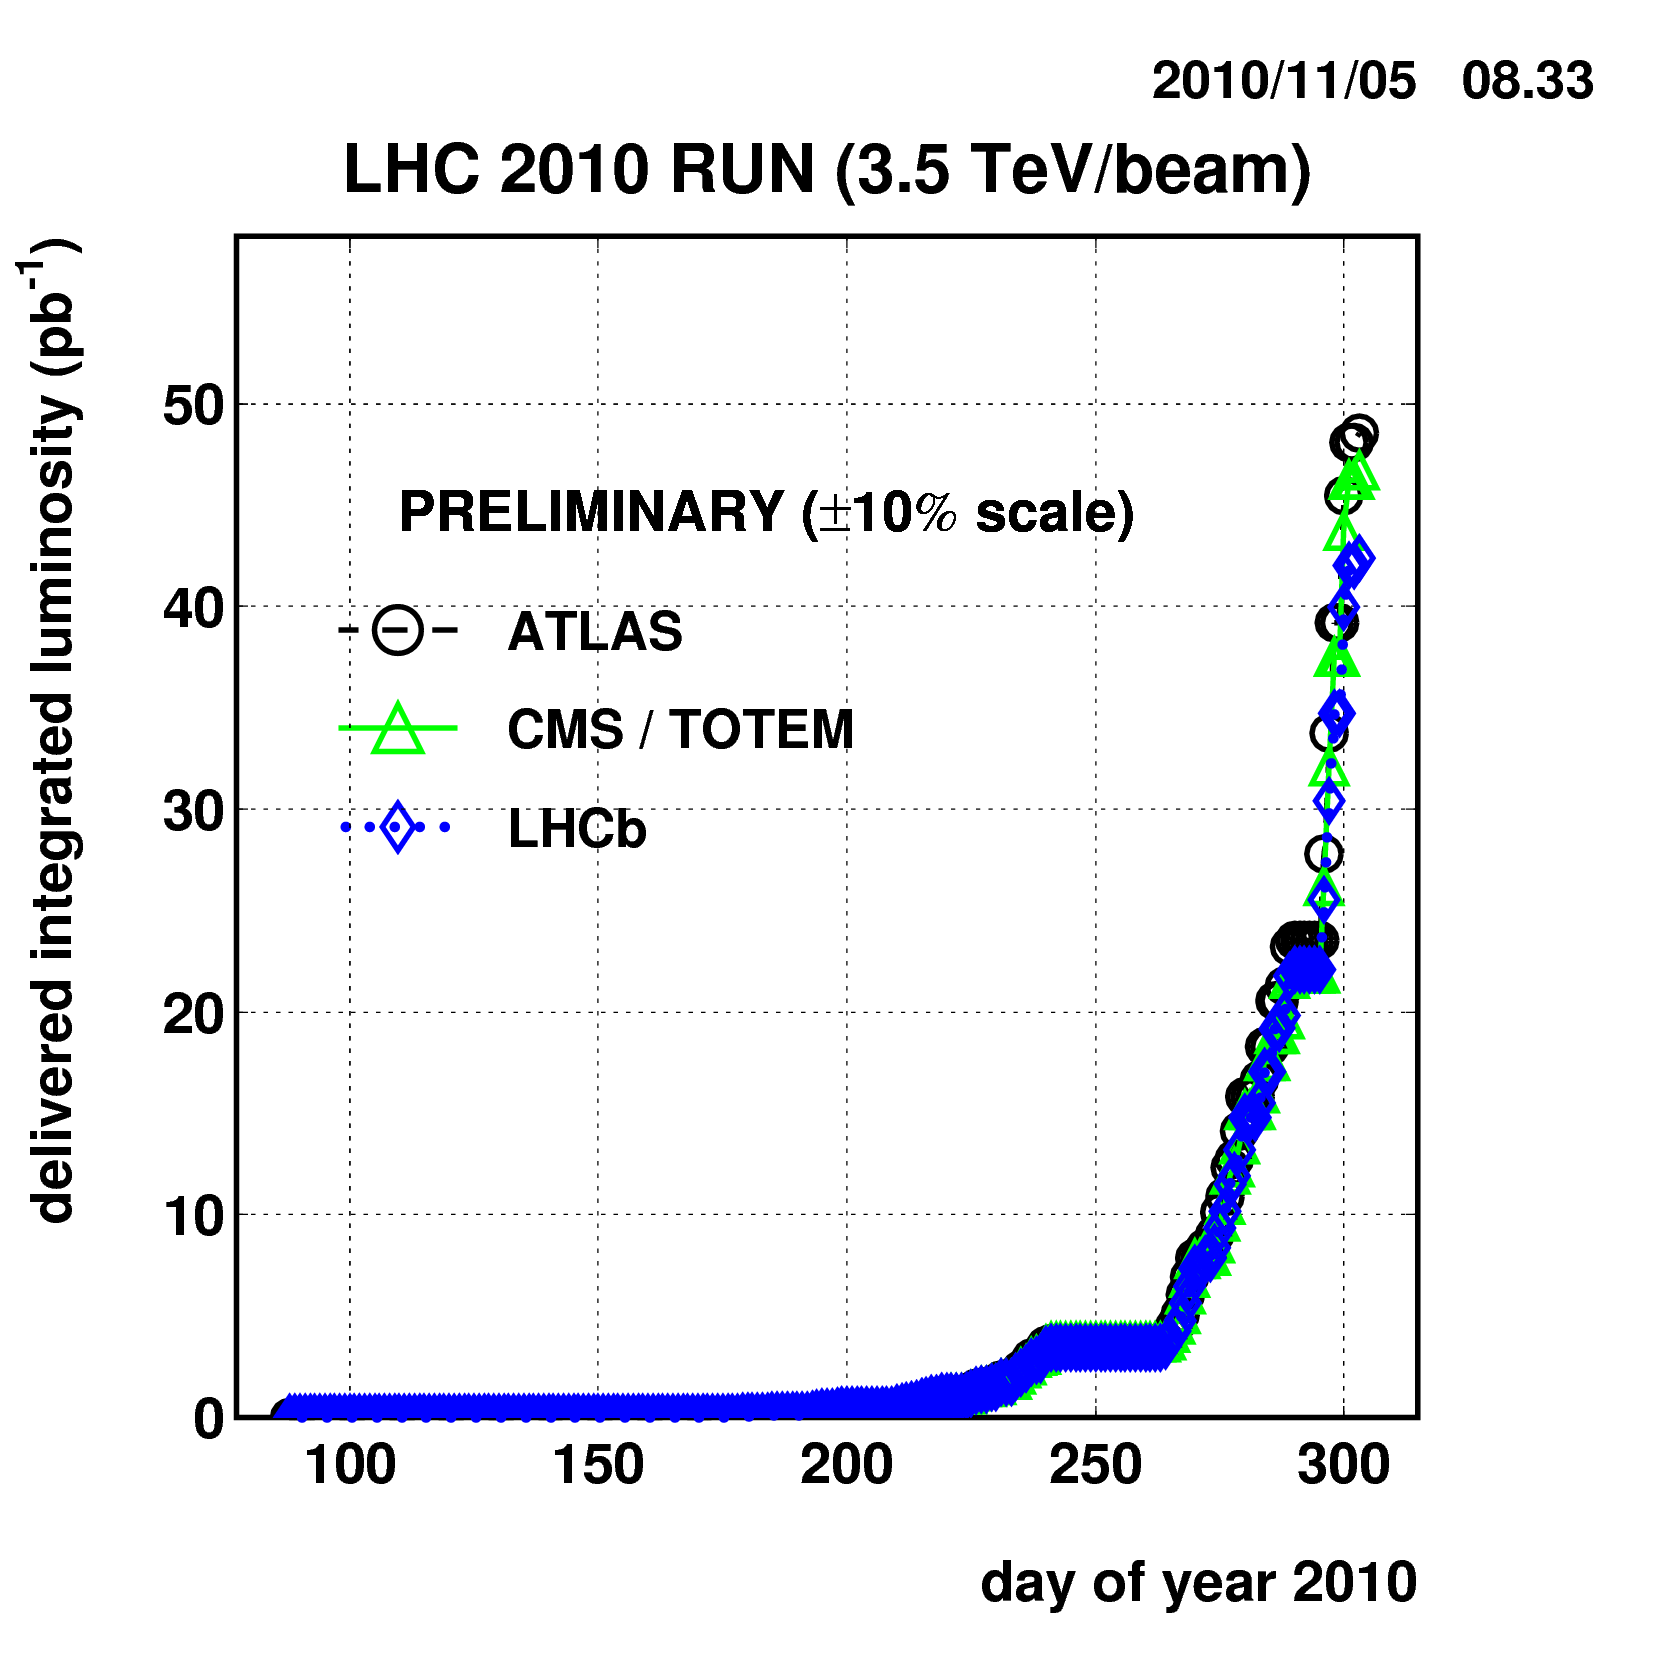
\includegraphics[width=0.49\textwidth]{Experiment/2010_lhc_luminocity.png}
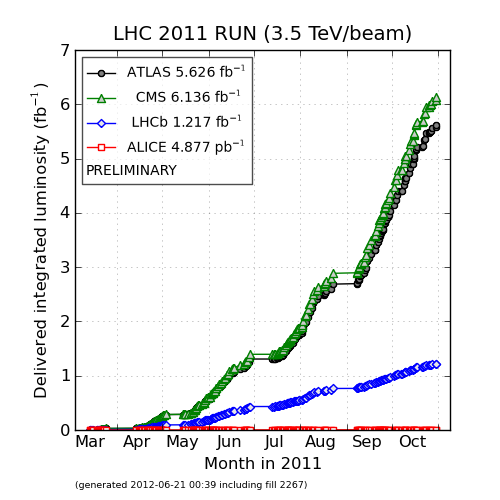
\includegraphics[width=0.49\textwidth]{Experiment/2011_lhc_luminocity.png}
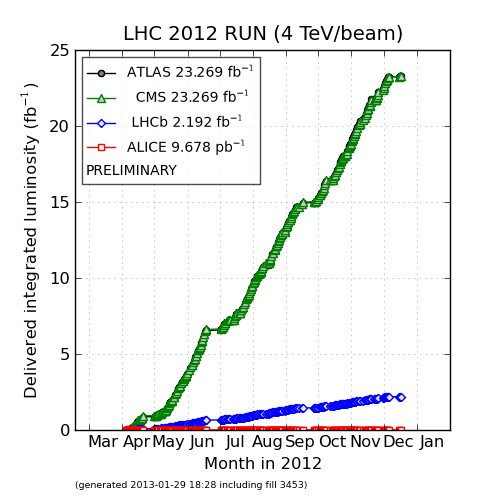
\includegraphics[width=0.49\textwidth]{Experiment/2012_lhc_luminocity.png}
\caption{Integrated luminosity delivered by the LHC to each experiment in 2010 to 2012.~\cite{lhc_lumi_plots}}
\label{fig:lhc_luminocity}
\end{figure}



%http://lpc.web.cern.ch/lpc/   %These are the LHC luminocity plots


%\subsection{Subsection heading}

%\subsubsection{Subsubsection heading}


\section{The Compact Muon Solenoid}

As one of the two general purpose detectors at the LHC, the Compact Muon Solenoid (CMS) has a wide range of physics goals, with its main focus on the Higgs boson search. Also important are physics beyond the Standard Model, precision measurement of known physics processes, and more.  With these goals in mind, there are a number of requirements that a detector must have that are present in the CMS detector~\cite{Bayatian:922757}. These are summarized below:

\begin{itemize}
 \item
   High efficiency in muon, electron, and photon identification with excellent momentum resolution in the pseudo-rapidity region $|\eta| <$ 2.5.
 \item 
   Mass Resolution of approximately 1\% for di-muon, di-electron, and di-photon events.
 \item 
   The ability to determine the charge of muons and electrons.
 \item
   Charged particle momentum resolution and reconstruction efficiency in the inner tracker. 
 \item
   Ability to identify the primary and secondary vertices for off line tagging b-jet and $\tau$.
 \item
  $\pi_0$ rejection and efficient photon and lepton isolation.
 \item
   High performance trigger system to reduce the event rate to amounts that can be stored in real-time.
 \item
   A tracking detector with sufficient precision to limit the effects of event pile-up.
\end{itemize}


  The main parts of the CMS detector include the 3.8 T superconducting solenoid, muon system, electromagnetic calorimeter, and the tracking system \cite{CMSExperiment}.  The CMS experiment has a number of cylindrical layers which are perpendicular to the beam axis (these are referred to as the barrel), and at both ends there are detector disks which are orthogonal to the beam axis (referred to as the endcaps). A more detailed picture of the detector can be found in Figures~\ref{fig:CMScolaborationPoster} and~\ref{fig:CMS_Slice}.  Figure~\ref{fig:CMS_luminosity} shows the data collection efficiency of the CMS detector for 2010 to 2012~\cite{cms_lumi_plots}.



\begin{figure}[htb]
\centering
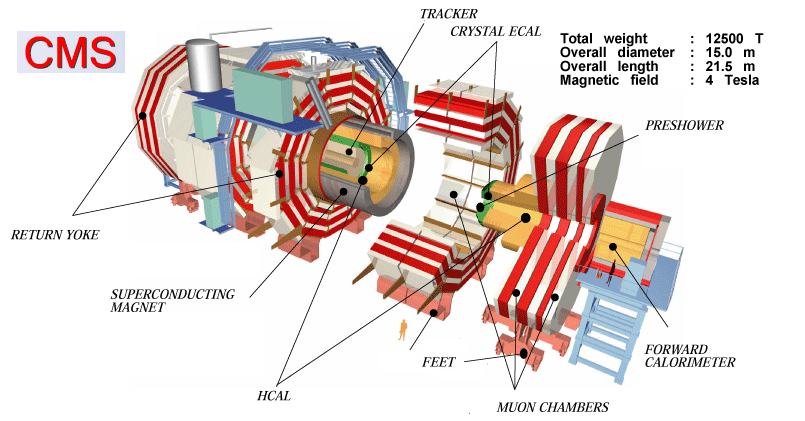
\includegraphics[width=0.99\textwidth]{Experiment/CMScollaborationPoster.png}
\caption{The CMS experiment.  HCAL stands for hadron calorimeter and ECAL stands for Electromagnetic calorimeter.}
\label{fig:CMScolaborationPoster}
\end{figure}

\begin{figure}[htb]
\centering
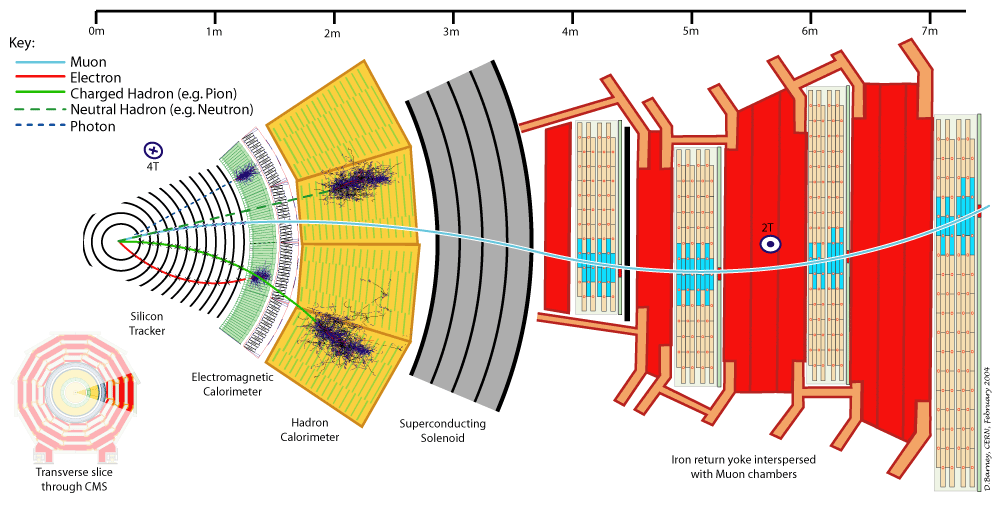
\includegraphics[width=0.99\textwidth]{Experiment/CMS_Slice.png}
\caption{A graphical slice of the CMS experiment.}
\label{fig:CMS_Slice}
\end{figure}


\begin{figure}[htb]
\centering
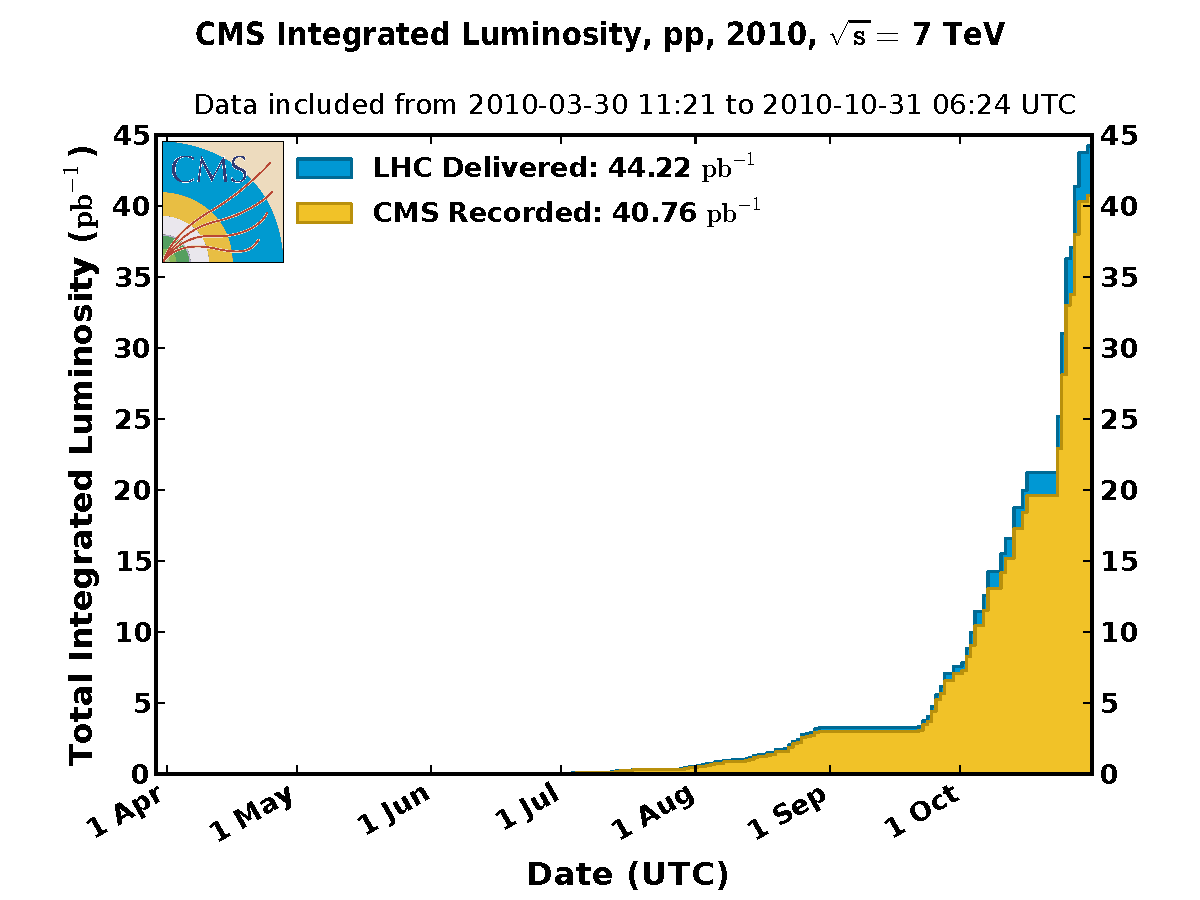
\includegraphics[width=0.49\textwidth]{Experiment/int_lumi_per_day_cumulative_pp_2010.pdf}
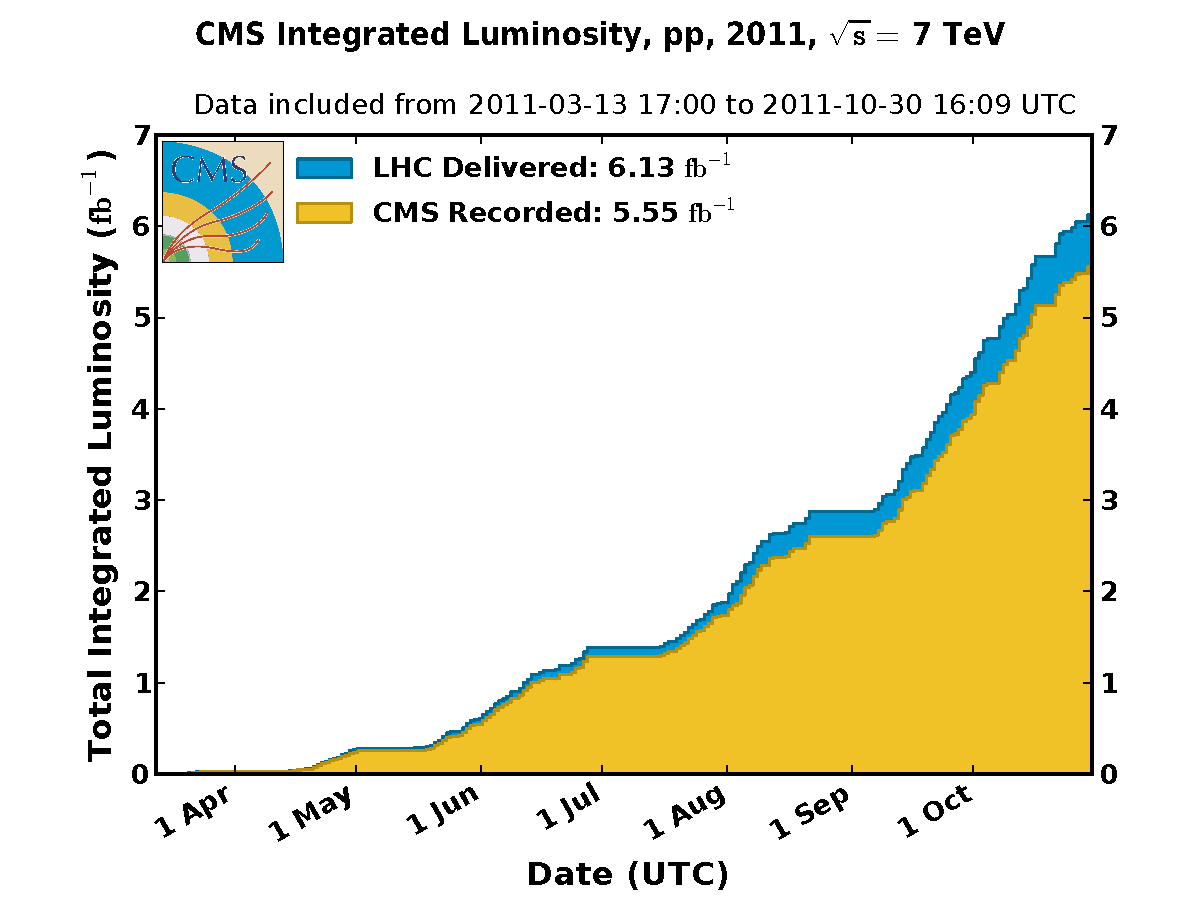
\includegraphics[width=0.49\textwidth]{Experiment/int_lumi_per_day_cumulative_pp_2011.pdf}
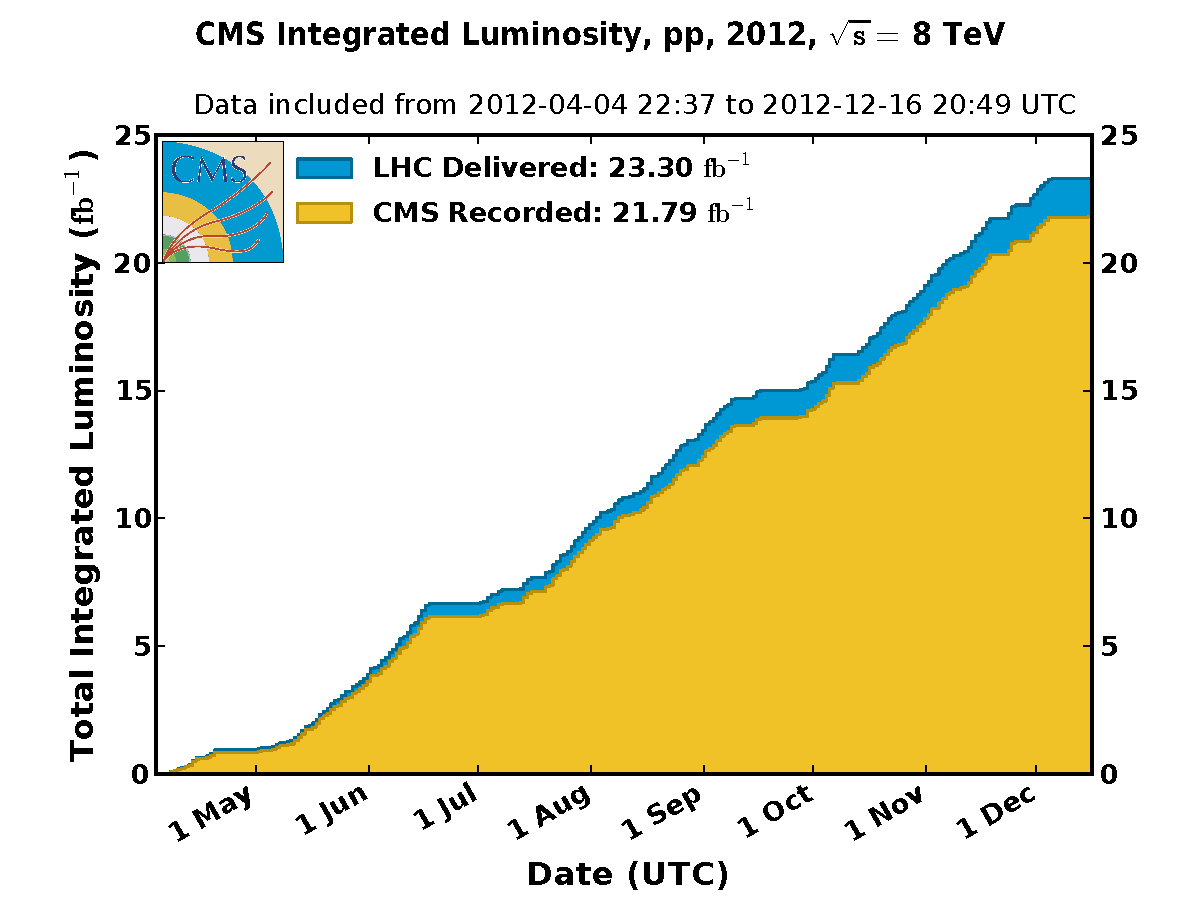
\includegraphics[width=0.49\textwidth]{Experiment/int_lumi_per_day_cumulative_pp_2012.pdf}
\caption{Total integrated luminosity for 2010 to 2012 delivered by the LHC and recorded by CMS.~\cite{cms_lumi_plots}}
\label{fig:CMS_luminosity}
\end{figure}

\subsection{CMS Subsections}
In the following sections a coordinate system will be used as illustrated in Figure~\ref{fig:CMS_detector_glossary}~\cite{Pandolfi_talk}.  Since the detector has a cylindrical shape around the beam axis, the beam axis is referred to as the z axis and a cylindrical coordinate system is used.

\begin{figure}[htb]
\centering
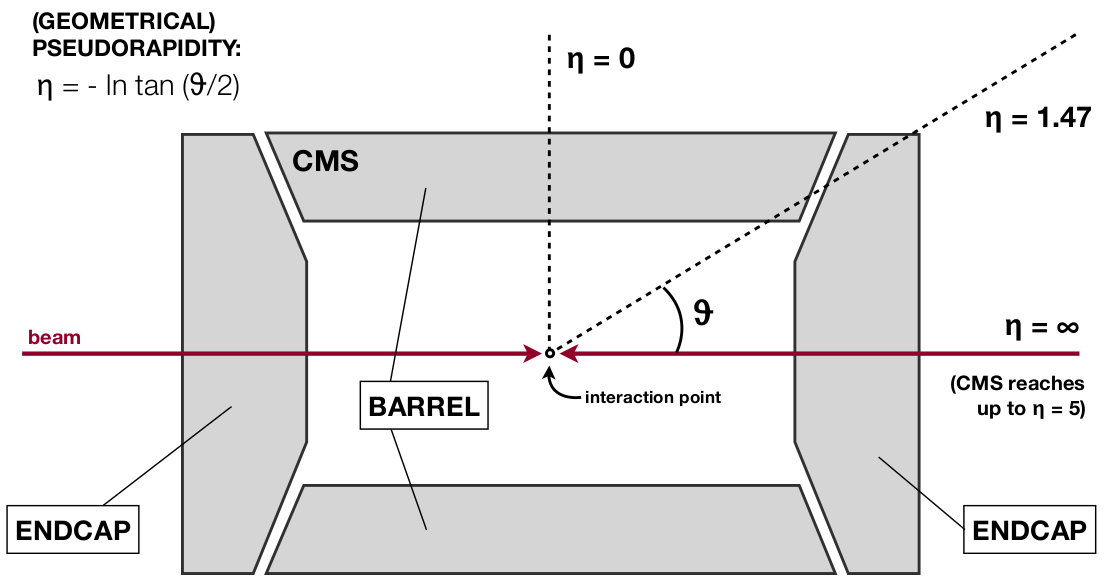
\includegraphics[width=0.99\textwidth]{Experiment/DetectorGlossary.png}
\caption{A CMS detector glossary of the cylindrical coordinate system used in this paper~\cite{Pandolfi_talk}.}
\label{fig:CMS_detector_glossary}
\end{figure}

It is useful to use the projection of momentum in the transverse plain because the net transverse momentum of collisions is close to zero.  We write:
\begin{equation} E_T = E \sin \theta = \dfrac{E}{\cosh\eta} \label{eq:transverse_energy}\end{equation}

When a particle is massless $E_T=p_T$.  Similarly, for the energies considered, the masses are negligible and we assume that $E_T=p_T$.

\subsubsection{Magnet}

To gain the resolution needed for the muon system, a large bending power of the detector is needed.  One way to achieve this goal is to use a solenoid.  The magnet in CMS is a 13 m long superconducting cylindrical Niobium-Titanium coil.  This coil has a diameter of 5.9 m with a uniform magnetic field of 3.8 T at its center.  The magnetic flux is returned by a double duty iron yoke support structure~\cite{Magnet_CMS}. This magnet can be seen in Figure~\ref{fig:CMS_solenoid_magnet}~\cite{cms_solenoid_magnet}.

\begin{figure}[htb]
\centering
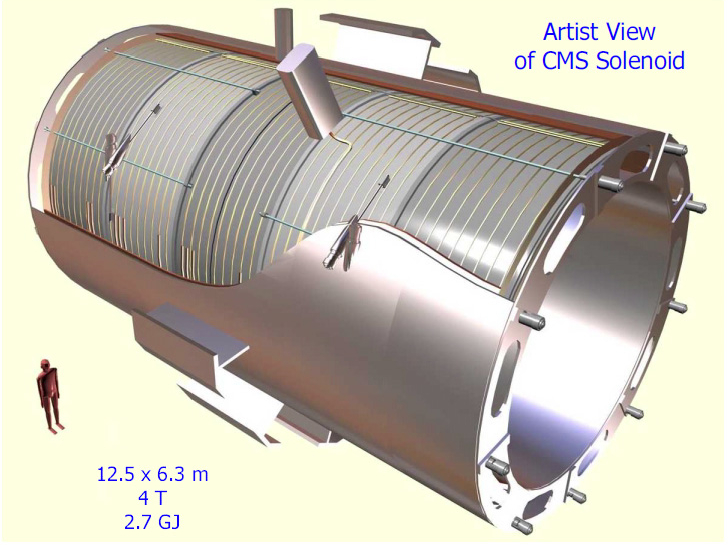
\includegraphics[width=0.59\textwidth]{Experiment/CMS-solenoid-magnet.jpg}
\caption{CMS solenoid magnet.~\cite{cms_solenoid_magnet}}
\label{fig:CMS_solenoid_magnet}
\end{figure}


\subsubsection{Tracker}
The tracker is the detector system that is closest to the primary interaction.  Its primary goal is to reconstruct the tracks of charged particles with extremely high precision both in position and momentum. The goal is greater than 95\% for electrons and muons and greater than 90\% for jets. It is also able to identify both the primary and secondary vertices.  Vertices are defined as the origin that a group of tracks share together. All these must be achieved in the extreme environment that is created by the LHC collisions~\cite{cms_trakcer_project}.

The previous requirements facilitated the choice of using a large silicon tracker~\cite{cms_trakcer_project}.  The tracker has three regions that are built differently because of the change in particle flux.  The closest region is the pixel detector where the particle flux is at a maximum.
%is about $10^7/s$.
In the intermediate regions, the flux has dropped sufficiently to be able to use silicon micro-strips.  In the outer region, again the particle flux is even lower which allows larger silicon micro-strips to be used.  This layout of the tracker can be seen in Figure~\ref{fig:CMS_tacker}~\cite{2010JInst...5.6007S}.

\begin{figure}[htb]
\centering
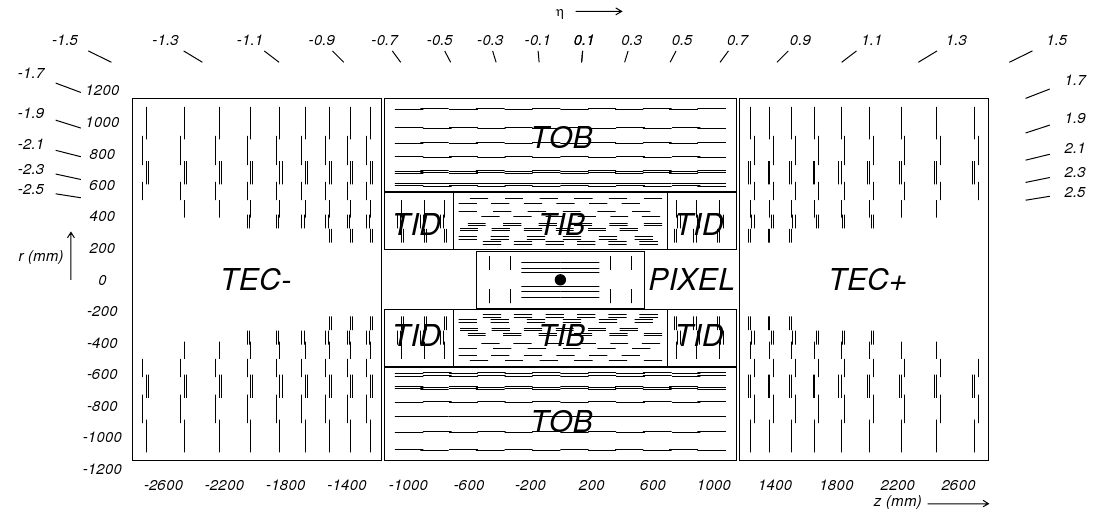
\includegraphics[width=0.69\textwidth]{Experiment/fig_cmstracker.png}
\caption{View of the CMS tracker in the rz-plane. Each line in the strip tracker represents a silicon strip detector, whereas lines in the pixel detector represent ladders and petals on which the detectors are mounted in the barrel and endcaps, respectively.~\cite{2010JInst...5.6007S}}
\label{fig:CMS_tacker}
\end{figure}

\subsubsection{The Calorimeters}

The CMS detector has two calorimeters, an electromagnetic calorimeter and a hadronic calorimeter. The electromagnetic calorimeter allows the precise measurement of both photon and electron energies.  The electromagnetic calorimeter is hermetic and homogeneous and made of 61,200 lead tungstate scintillating crystals in the barrel and 7,324 crystals in the two endcaps~\cite{ECAL_report}.

The lead tungstate crystals have a number of important features as listed below:
\begin{itemize}
  \item
    Short radiation length (0.89 cm) that allows a compact calorimeter into the small space available.
  \item
    Very fast light emission (5 ns for primary and 15 ns for secondary) since LHC bunch crossings are 25 ns.
    \item
      Radiation hard at a level to allow several decades of high luminosity operation.
    \item
      Excellent position tracking because of the small shower containment. 
\end{itemize}

One downside is that light yield is low and therefore photo detectors with a high gain must be used.  Figure~\ref{fig:CMS_ecal_quadrant}~\cite{ECAL_report} shows a longitudinal cross section of the ECAL. Any dead areas where there is not detection significantly degrades the total energy measurement and hurts the missing transverse energy (MET) calculations. Figure~\ref{fig:CMS_ecal_crack} shows the gap which was designed to minimize these problems~\cite{ECAL_report}. The overlap region $1.4442 < |\eta| < 1.566$ is excluded for certain measurements in the analysis for electrons.

\begin{figure}[htb]
\centering
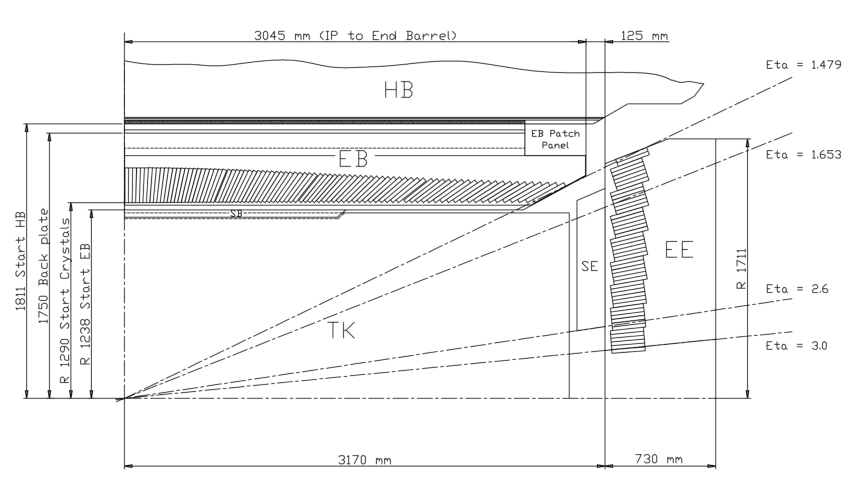
\includegraphics[width=0.69\textwidth]{Experiment/ECAL_quadrant.pdf}
\caption{Longitudinal section of the electromagnetic calorimeter (one quadrant).~\cite{ECAL_report}}
\label{fig:CMS_ecal_quadrant}
\end{figure}

\begin{figure}[htb]
\centering
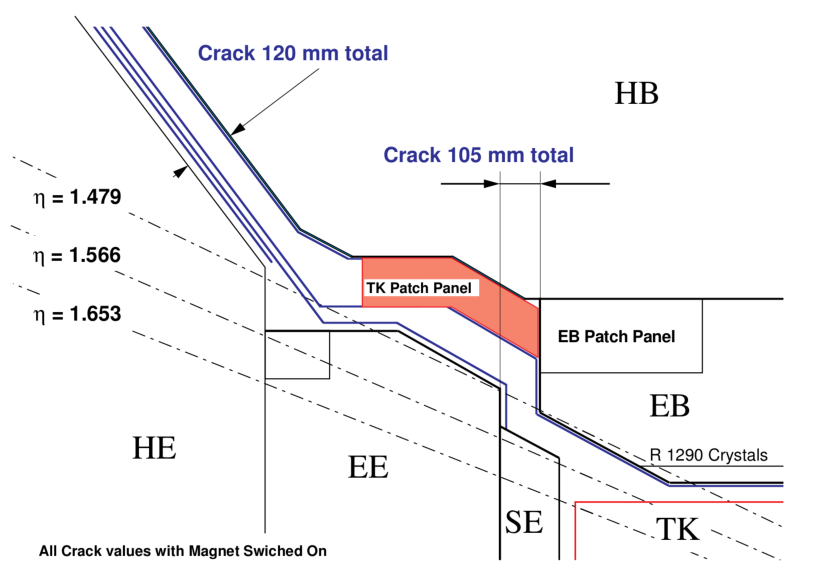
\includegraphics[width=0.69\textwidth]{Experiment/ECAL_TDR_crack.pdf}
\caption{The barrel and endcap transition region.~\cite{ECAL_report}}
\label{fig:CMS_ecal_crack}
\end{figure}

The hadronic calorimeter~\cite{HCAL_report} detects quarks, gluons, and neutrinos.  This is done by measuring the energy and position of particle jets as well as the missing transverse energy (MET).  In conjunction with the other systems, it also helps with the identification of electrons, photons, and muons with the ECAL and muon systems.  The central hadron calorimeter is a sampling calorimeter. The hadron calorimeter is made of 4mm thick plastic scintillator tiles. It uses brass as the absorber material. A quarter slice of the HCAL can be seen in Figure~\ref{fig:CMS_hcal}~\cite{Chatrchyan:2009hw}.

\begin{figure}[htb]
\centering
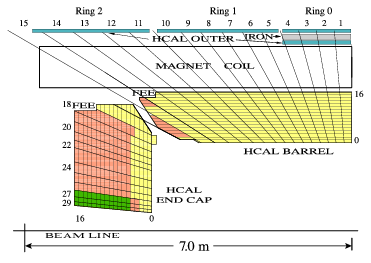
\includegraphics[width=0.69\textwidth]{Experiment/fig_HCALdiagram.png}
\caption{A quarter slice of the CMS HCAL detectors. The right end of the beam line is the interaction point. FEE denotes the location of the Front End Electronics for the barrel and the endcap. In the diagram, the numbers on the top and left refer to segments in $\eta$, and the numbers on the right and the bottom refer to scintillator layers. Colors/shades indicate the combinations of layers that form the different depth segments, which are numbered sequentially starting at 1, moving outward from the interaction point. The outer calorimeter is assigned depth 4.~\cite{Chatrchyan:2009hw}}
\label{fig:CMS_hcal}
\end{figure}


\subsection{The CMS Trigger System}

At the high luminosity achieved at the LHC, there is the drawback that several of the interactions overlap in the same bunch crossing. Also there is overlap from different bunch crossing because of the limited speed of the detector response and data read-out.  These effects are known as pile-up.  In addition to pile-up difficulties, there is an extreme amount of data produced from the collisions at CMS. With a luminosity of $10^{34}cm^{-2}s^{-1}$, there are roughly $10^9$ interactions per second.  With the typical event size of 1 MB, all collisions cannot be recorded and with the majority of interactions not interesting for the CMS physics program, there needs to be a way to choose which events to record.  This is done with the triggering system to reduce the recorded rate to approximately 100 Hz. There are technical difficulties in the handling, processing, and storing of this data. These difficulties make the real time selection and recording of important events (the trigger) very important~\cite{Bayatyan:706847}.

The CMS trigger has two levels.  The Level 1 (L1) trigger is a hardware trigger.  The full data is stored in the pipelines for processing while waiting for the trigger decision.  If the L1 accepts the decision, then the data is moved to the software based High Level Trigger (HLT).  The HLT reduces the output rate to around 100 Hz. The HLT software has a set of algorithms which give complete freedom in deciding which data to access.  To free up processing, there are three virtual trigger levels.  The first only uses the muon and calorimeter data, the second adds the pixel seeds, and the final step uses the full event information. Both L1 and HLT triggers have changed as the LHC environment changed during the luminosity increases.

The Level 1 trigger is used to choose hard scattering from processes like Higgs decays, $WW$ scattering, supersymmetry, and more.  This system is based on custom electronics.  It uses the identification of photons, electrons, muons, jets, and missing transverse energy. A diagram of the L1 trigger system is shown in Figure~\ref{fig:l1triggeroverview}~\cite{Bayatyan:706847}. The physics requirements for the L1 trigger are as follows~\cite{Bayatyan:706847}:
\begin{itemize}
  \item
    The CMS trigger system should be capable of selecting leptons and jets over the pseudo-rapidity range $|\eta| < 2.5$, with an efficiency which is very high, above a selected threshold in transverse momentum.
  \item
    For the single lepton triggers, it is required that the trigger is fully efficient ($>$ 95\%) in the pseudo-rapidity range $|\eta| < 2.5$, with a threshold of $p_T> 40$ GeV.
  \item
    For the dilepton trigger, it is required that the trigger is fully efficient ($>$ 95\%) in the pseudo-rapidity range $|\eta| < 2.5$ with thresholds of $p_T> 20$ and 15 GeV for the first and second leptons respectively.
  \item
    Single photon and diphoton triggers are required to have thresholds similar to those of the leptons.
  \item
    Single and multiple jet triggers are required with a well defined efficiency over the entire rapidity range $|\eta| < 5$ in order to reconstruct jet spectra that overlap with data attainable at lower energy colliders, such as the Tevatron. For higher transverse momenta, the jet trigger should also be fully efficient.
  \item
    A missing transverse energy trigger with a threshold of about 100 GeV is required.
\end{itemize}

\begin{figure}[htb]
\centering
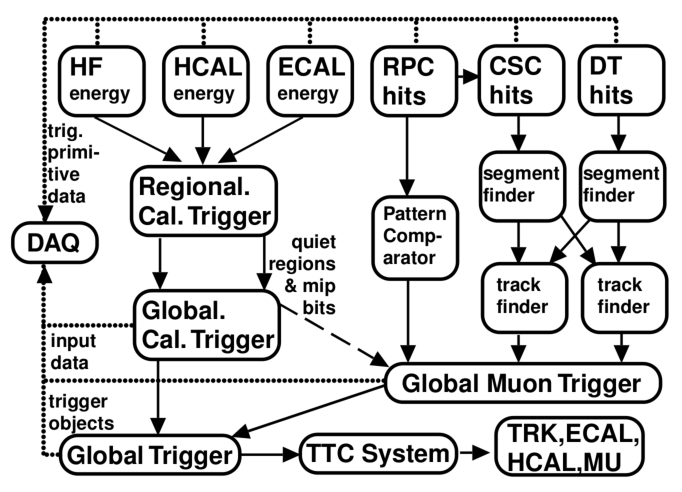
\includegraphics[width=0.69\textwidth]{Experiment/l1trigger.pdf}
\caption{Overview of Level 1 Trigger.~\cite{Bayatyan:706847}}
\label{fig:l1triggeroverview}
\end{figure}

The High-Level trigger is a software system with maximum flexibility for selection and the changing environment of the LHC~\cite{Cittolin:578006}.  It takes the output from the Level 1 trigger to do a rough event reconstruction.  With this rough reconstruction the HLT makes the decision to either reject the event or pass it through to a more detailed reconstruction.  This is decided by a number of criteria that are collectively used to create data sets.  These are designed to meet the various physics' goals that CMS was designed to study. Common requirements are high $p_T$ lepton pairs, or large amounts of MET.%$M_T^{miss}$.
